\documentclass[12pt]{article}
\usepackage{rocca-homework}

\title{MAT 141 Homework 5}
\author{Lucas Vas}
\date{12/15/2023}

\begin{document}

\maketitle

  \begin{problem}{Chapter 10.1 Question 28}
    When there are at least 2 people in a party, that party will have at least 2 mutual friends or strangers.
    We can draw a graph showing this, where each person is a vertex and each ''friendship'' is symbolized as
    an edge:
    \begin{center}
      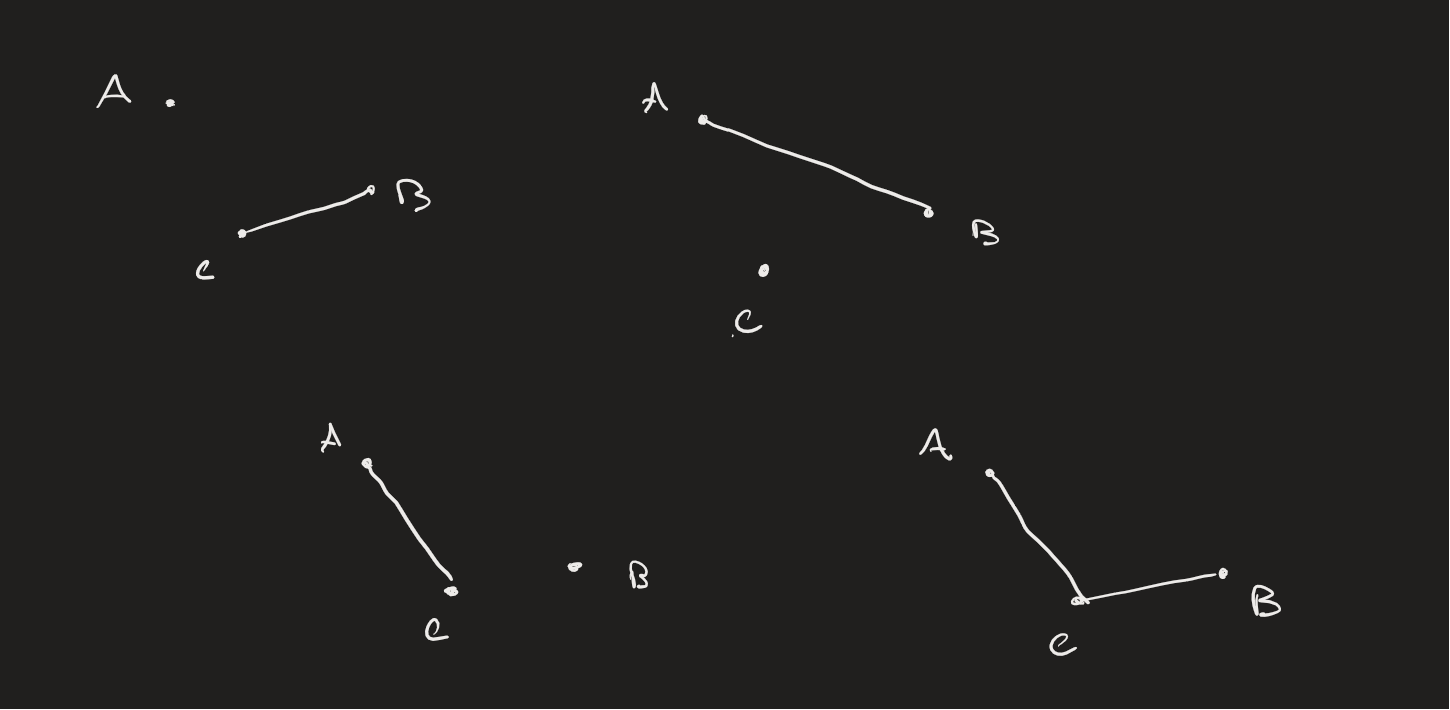
\includegraphics[width=8cm]{2friends.png}
    \end{center}
    In these graphs, we can see that there are some isolated vertices, indicating that there are some people
    who have no friends (at this party, of course). We can also see that there are some vertices with degree
    1 or more, indicating that there are some people with at least 1 friend. There are always at least 2 people
    that are friends in all of these graphs, so the statement is true.

    I could have also drawn a grpah in which none of the vertices are connected, which would indicate that 
    there are no mutual friends within said party. However, the statement still holds true because at this point
    there are at least 2 mutual strangers.
  \end{problem}

  \begin{problem}{Chapter 10.1 Question 42}
    In this problem, we are asked to find a Hamiltonian circuit in a weighted graph which minimizes the total
    distance travelled. My implementation of this question is shown in this graph:
    \begin{center}
      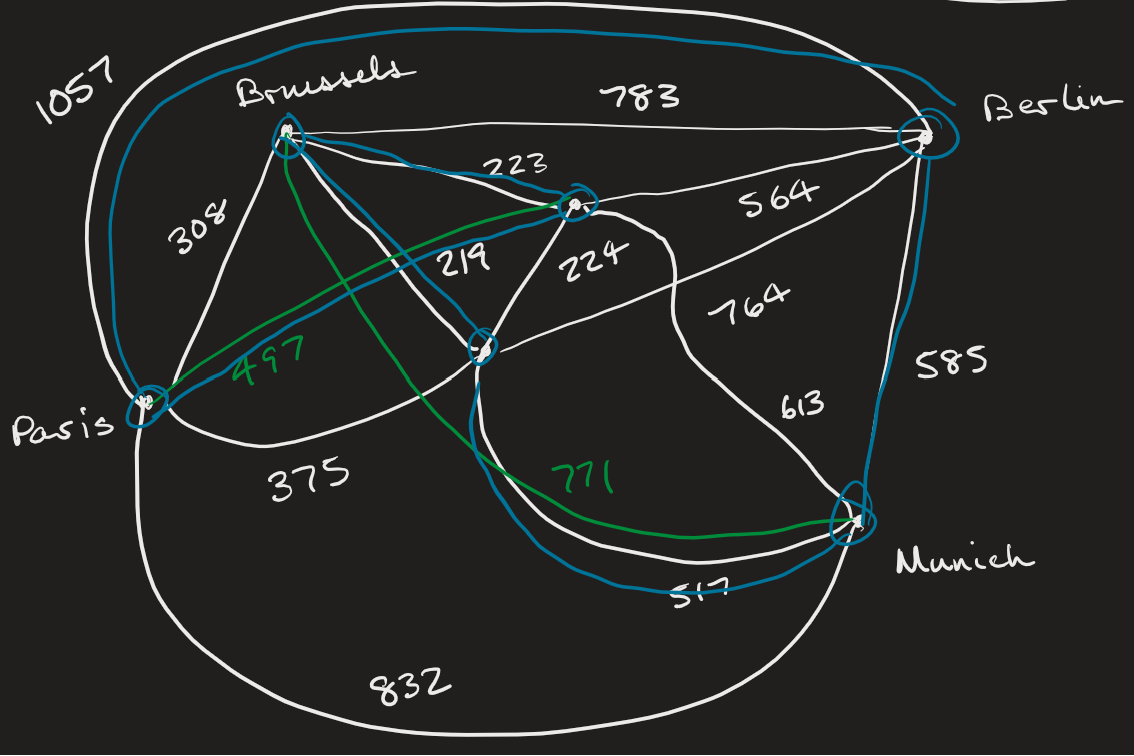
\includegraphics[width=8cm]{cities.png}
    \end{center}
    The total distance travelled is 3098. I found the circuit by hand, by choosing the shortest edge at each
    vertex towards another that has not been visited yet. I started at Berlin. The path is:
    \begin{equation*}
      \text{Berlin} \rightarrow \text{Munich} \rightarrow \text{Luxembourg} \rightarrow \text{Brussels} \rightarrow \text{Dusseldorf} \rightarrow \text{Paris} \rightarrow \text{Berlin}
    \end{equation*}
  \end{problem}

  \begin{problem}{Chapter 10.4 Question 24}
    Given a connected graph with a leaf vertex, we can remove that leaf and its edge and still have a connected graph.
    The first graph would look roughly like this:
    \begin{center}
      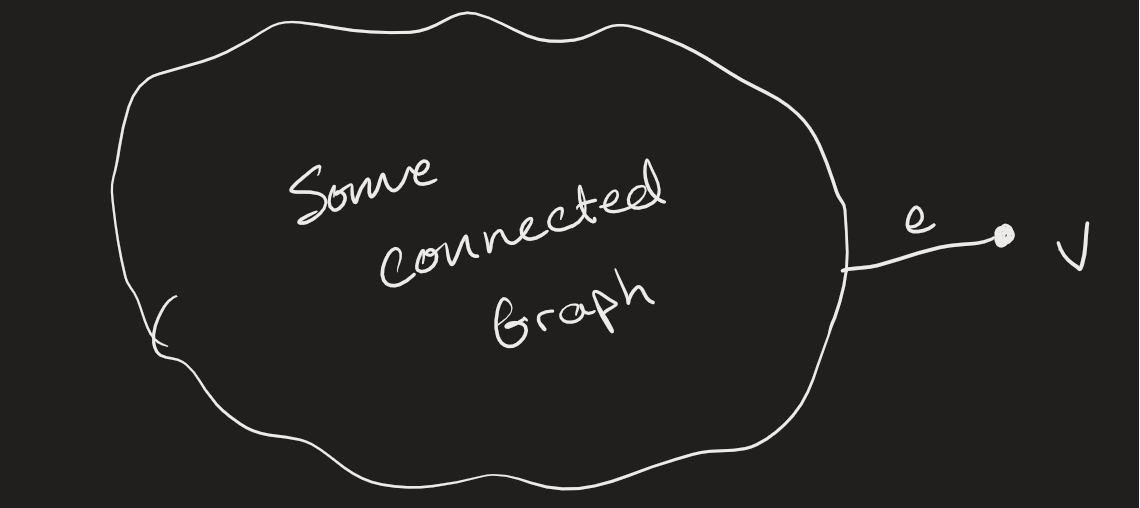
\includegraphics[width=8cm]{connected1.png}
    \end{center}
    I have abbreviated the graph due to the fact that most of it is irrelevant. The leaf vertex is labelled as $V$ and the
    edge is labelled as $e$. The second graph would look roughly like this:
    \begin{center}
      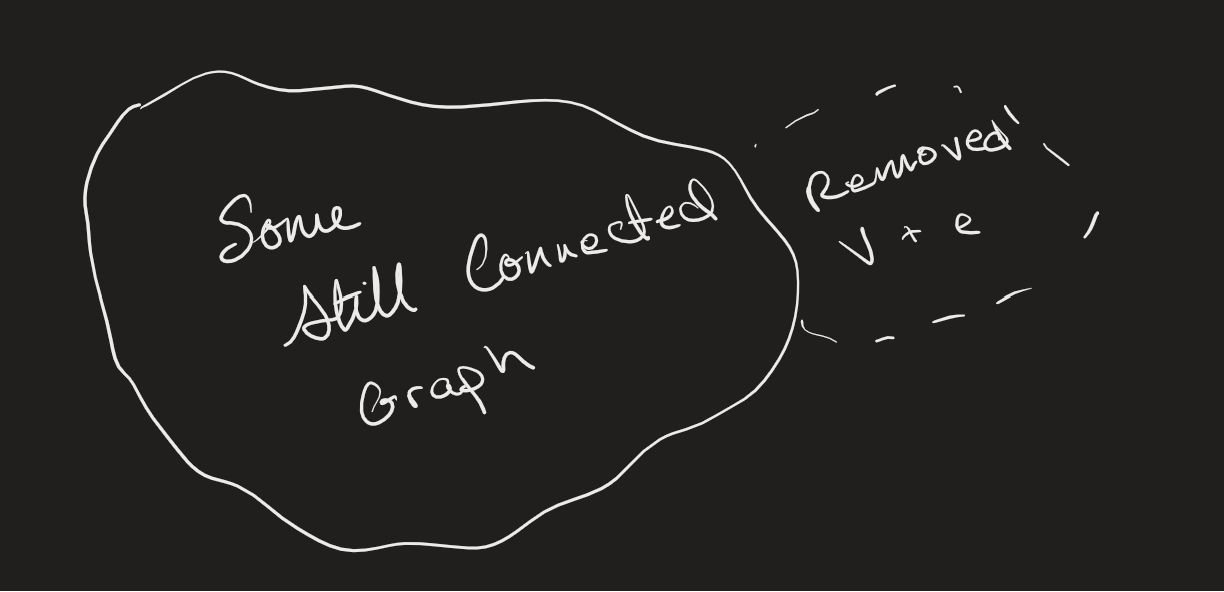
\includegraphics[width=8cm]{connected2.png}
    \end{center}
    As we can see, the graph would still be connected. This is because the leaf vertex, by definition of being a leaf, only
    has one edge. Removing that edge would remove the leaf vertex, but the graph would still be connected because the leaf
    vertex was only connected to one other vertex.
  \end{problem}

\end{document}
